% XCircuit output "schema_zakladna.tex" for LaTeX input from schema_zakladna.ps
\def\putbox#1#2#3#4{\makebox[0in][l]{\makebox[#1][l]{}\raisebox{\baselineskip}[0in][0in]{\raisebox{#2}[0in][0in]{\scalebox{#3}{#4}}}}}
\def\rightbox#1{\makebox[0in][r]{#1}}
\def\centbox#1{\makebox[0in]{#1}}
\def\topbox#1{\raisebox{-0.60\baselineskip}[0in][0in]{#1}}
\def\midbox#1{\raisebox{-0.20\baselineskip}[0in][0in]{#1}}
   \scalebox{0.8}{
   \normalsize
   \parbox{2.60335in}{
   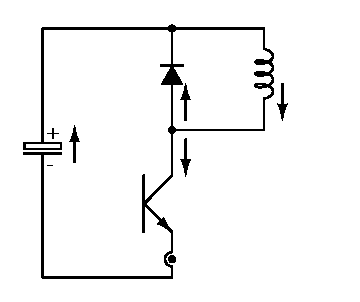
\includegraphics[scale=1.25]{schema_zakladna}\\
   % translate x=284 y=237 scale 0.28
   \putbox{1.45in}{0.99in}{1.20}{\llgic}%
   \putbox{1.45in}{1.49in}{1.20}{\llgiD}%
   \putbox{2.26in}{1.45in}{1.20}{\llgiL}%
   \putbox{0.52in}{1.14in}{1.20}{\llgiK}%
   } % close 'parbox'
   } % close 'scalebox'
   \vspace{-\baselineskip} % this is not necessary, but looks better
